\renewcommand*\contentsname{\begin{center}ЗМІСТ\end{center}}
\tableofcontents

\newpage

\begin{center}
\textbf{ПЕРЕЛІК УМОВНИХ ПОЗНАЧЕНЬ, СКОРОЧЕНЬ І ТЕРМІНІВ}
\end{center}

\hypertarget{term1}{Крос-платформенна мова програмування}
\hypertarget{term2}{Парсинг}
\hypertarget{term3}{.conllu}


\newpage

\begin{center}
\textbf{ВСТУП}
\end{center}

\newpage

\section{ПОСТАНОВКА ЗАДАЧІ}

\section{???АНАЛОГИ???}

\section{ЗАСОБИ РОЗРОБКИ}
Галузь інформаційних технологій рушила далеко вперед за останні декілька десятків років.
У тому числі в питанні засобів розробки. 


Зараз існує багато інструментів, які покликані
полегшити та покращити досвід написання коду та усі цикли розробки програмного забезпечення
в цілому. З'явилося чимало мов програмування загального призначення,
які все ж зайняли свої певні ніші й використовуються переважно в якійсь одній галузі,
незважаючи на своє загальне призначення. Оскільки ресурси розробників цих мов не необмежені,
вони фокусуються на конкретних функціях та особливостях і реалізовують саме їх. Таким чином,
навіть мови загального призначення відрізняються одна від одної і підходять краще під ті, чи інші задачі. Тому дуже важливо не бездумно користуватися найпростішим, чи тим інструментом,
який ти знаєш краще, а обирати і вивчати ті, які найкраще підходять під поставлену задачу.

\subsection{Мова програмування Python}
Для написання цієї роботи використовувалася мова програмування Python. Це інтерпретована
об'єктно-орієнтована мова програмування високого рівня зі строгою динамічною типізацією.
Ця мова відома, перш за все, за свою відносну простоту та низький поріг входу,
а також за високий темп розробки, внаслідок свого динамічного та інтерпритованого характеру.
Оскільки ця мова інтерпритується віртуальною машиною, а не компілюється під конкретну
операційну систему, це робить її також \hyperlink{term1}{крос-платформенною}.
Але основна причина чому мова Python чудово підходить для задач обробки природної мови
та статистичного аналізу - це велика спільнота науковців та розробників, які створили чималу
кількість бібліотек та інструментів які підвищують рівень абстракції і дозволяють сфокусуватися
на предметі дослідження і не відволікатися на низькорівневі речі, як-от
\hyperlink{term2}{парсинг} вихідних файлів.

-- SMTH ABOUT UNIT TESTS--

\subsubsection{Пакетний менеджер Pip}
щось про піп

\subsubsection{Інтегроване середовище розробки PyCharm}
Як основне середовище розробки використовувався рушій PyCharm, розроблений компанією JetBrains

\begin{figure}[h]
    \centering
    \noindent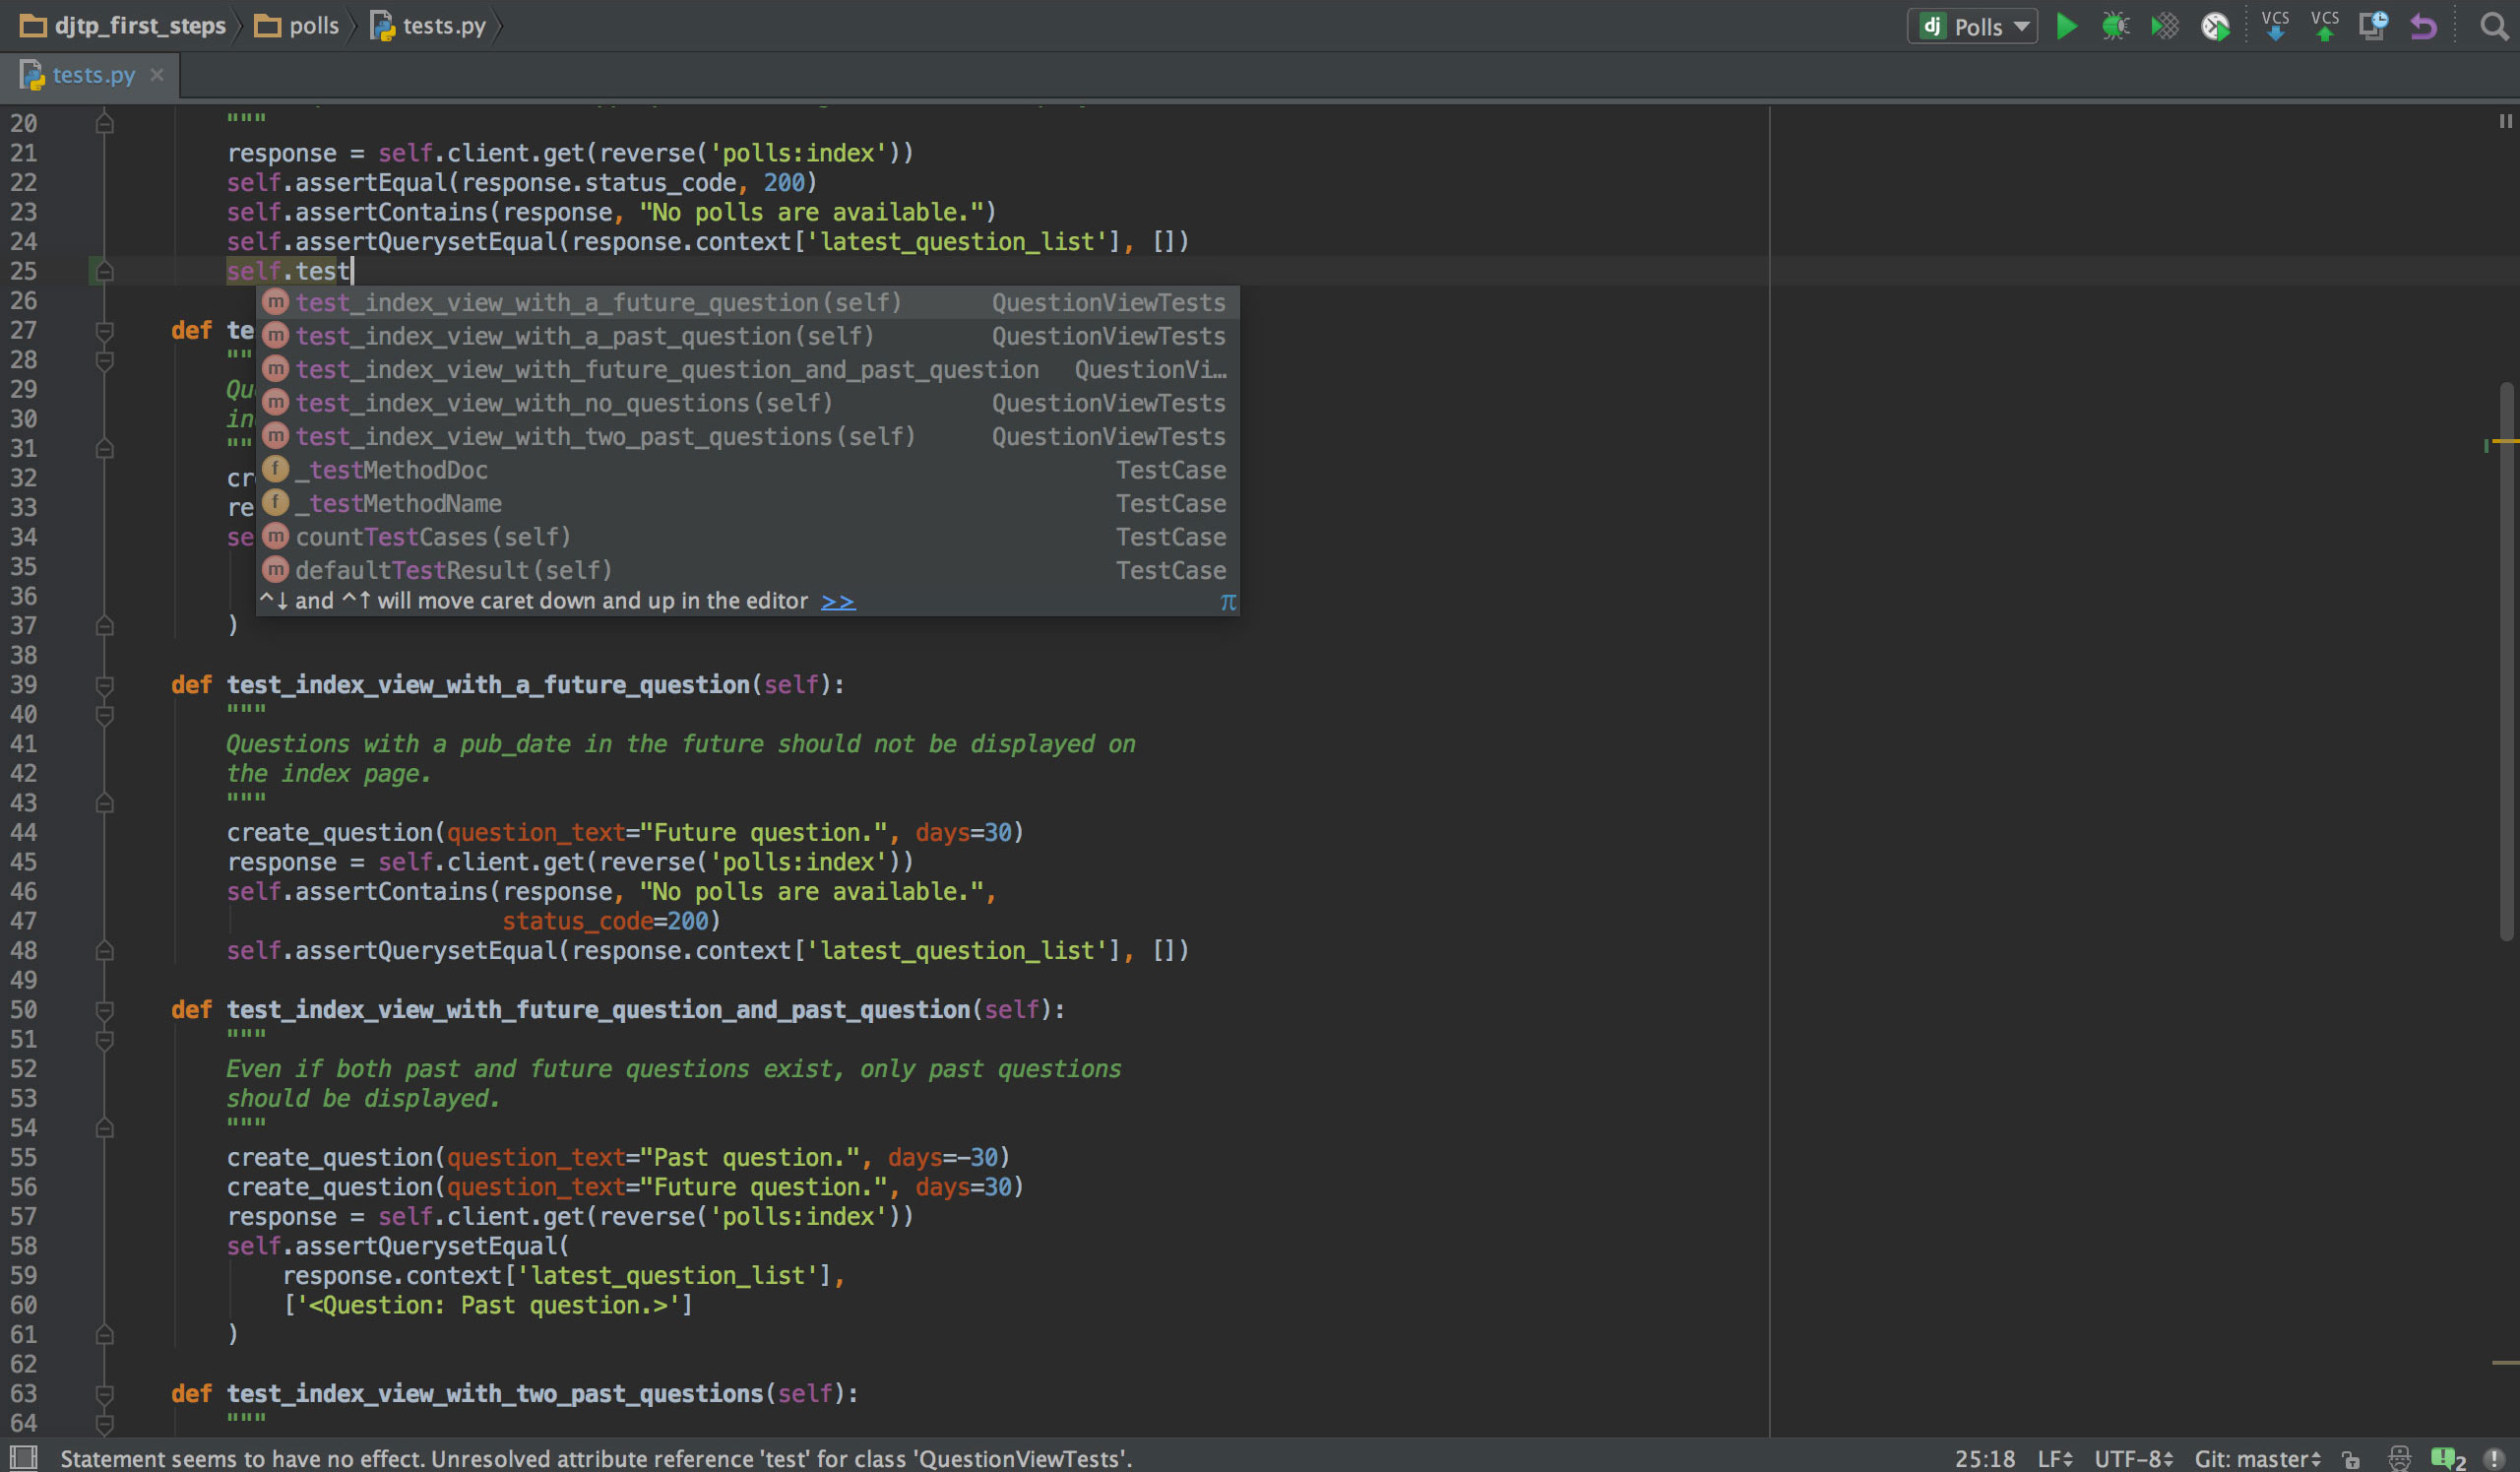
\includegraphics[width=\linewidth]{pycharm.jpg}
    \caption{a nice plot}
    % \label{fig:mesh1}
\end{figure}


\subsection{Система контролю версій Git}
% \subsubsection{Інтернет хостинг GitHub}